\documentclass[11pt,a4paper]{article}

\usepackage[margin=1in]{geometry}
\usepackage{amsmath,amssymb}
\usepackage{booktabs}
\usepackage{graphicx}
\usepackage{xcolor}
\usepackage[numbers]{natbib}
\usepackage[colorlinks=true,linkcolor=blue!50!black,citecolor=blue!50!black,urlcolor=blue!50!black]{hyperref}

\newcommand{\todo}[1]{\textcolor{red}{[TODO: #1]}}
\newcommand{\sbr}[1]{\texttt{#1}}


\title{\LARGE\textbf{Learning-Augmented Branch-and-Bound:}\\[4pt]
\large\textbf{Imitating Strong Branching with Cheap Features in SCIP}}
\author{Mohammed Abo Oraig \\ \small Independent research \\ \small \texttt{mohammed-abo-oraig@etud.univ-tln.fr}}
\date{}


\begin{document}
\maketitle
 
\begin{abstract}
The branching rule largely determines the size of a branch-and-bound tree. Strong branching builds small trees but is expensive; cheap rules such as pseudocost branching are fast but less informed. We train a gradient-boosted ranking model to imitate strong branching from 19 inexpensive features of the current optimization state, and plug it into SCIP as a custom branching rule through PySCIPOpt. On random set-covering instances, with cuts and presolve disabled, the learned rule solves instances in 39--48\% less time than SCIP's reliability pseudocost branching (on 50 unseen test instances and on 30 larger ones) and about four times faster than most-fractional branching (test instances). Against plain pseudocost branching it builds about 20\% smaller trees but is not faster. Feature extraction and model scoring cost 8--12\% of the solve time, and a rough estimate suggests that even removing this overhead entirely would give at most a few percent. We report the overhead breakdown, generalization to larger instances, and the limits of this small study.
\end{abstract}
 
\section{Introduction}
Branch-and-bound solves mixed-integer programs by repeatedly splitting the problem on a fractional integer variable. Which variable to split on---the \emph{branching decision}---has a large effect on the number of nodes explored. \emph{Strong branching} evaluates every candidate by solving two linear programs (LPs) per candidate and produces very small trees, but it is too slow to use at every node; practical solvers combine it with cheap pseudocost statistics, as in reliability branching \citep{achterberg2005branching}. A line of work asks whether a model can \emph{learn} to imitate strong branching at a fraction of its cost, using hand-crafted features \citep{khalil2016learning} or graph neural networks \citep{gasse2019exact}; see \citet{bengio2021machine} for a survey.
 
This report is a small, self-contained empirical study of this idea. We keep the learning component deliberately simple---a gradient-boosted ranker on cheap features---and focus on a careful end-to-end evaluation inside a real solver. We ask three questions:
\begin{enumerate}
  \item[\textbf{Q1}] Does the learned rule beat classical branching rules in nodes, time and optimality gap on unseen instances?
  \item[\textbf{Q2}] Does it generalize to instances larger than those seen in training?
  \item[\textbf{Q3}] What does the learned policy cost, and where does that cost come from?
\end{enumerate}
Our main findings are: the learned rule is clearly better than most-fractional and reliability pseudocost branching under our protocol; it builds smaller trees than pseudocost branching but is not faster than it; and its overhead is dominated by feature extraction, not by the model. Code and data-generation scripts are available at \url{https://github.com/AboOraig/learned-augmented-optimization}.
 
\section{Background}
Let a node of the tree have LP relaxation value $z$ and let $C$ be the set of integer variables with fractional LP value. We use four branching rules.
\paragraph{Strong branching.} For each $j\in C$, solve the two child LPs; let $\Delta_j^-,\Delta_j^+\ge 0$ be the resulting increases of the LP bound. The variable maximizing the product score $\max(\Delta_j^-,\epsilon)\cdot\max(\Delta_j^+,\epsilon)$ is selected. This is the expert we imitate.
\paragraph{Pseudocost branching.} Replaces the LP solves by running averages of the per-unit bound improvement observed in past branchings of each variable; very cheap, but uninformed for variables branched on rarely.
\paragraph{Reliability pseudocost branching.} SCIP's default rule (\sbr{relpscost}) \citep{achterberg2005branching}: uses pseudocosts but falls back to strong branching on candidates whose pseudocosts are not yet reliable.
\paragraph{Most fractional branching.} Selects the variable whose LP value is closest to $0.5$ (\sbr{mostinf} in SCIP); trivially cheap, usually builds large trees.
 
\section{Method}
\subsection{Instances}
We use random set-covering problems $\min\{c^\top x : Ax\ge \mathbf 1,\ x\in\{0,1\}^n\}$ in the spirit of \citet{balas1980set}: density $5\%$, every row covered by at least two columns, every column covering at least one row, integer costs uniform in $\{1,\dots,100\}$. Training, validation and test instances have $500$ rows and $1000$ columns; a separate transfer set has $750$ rows and $1000$ columns and is used only for evaluation. All instance sets use disjoint random seeds.
 
\subsection{Collecting expert data}
A custom branching rule with the highest priority is called at every node. At the root and at each further node with probability $0.1$ (at most $30$ sampled nodes per instance) it computes the features of Section~\ref{sec:features} for a random subset of at most $60$ candidates and runs strong branching on them (LP iteration limit $100$ per probe). The candidate with the largest product score is recorded as the label, and the tree continues with that choice at sampled nodes; at all other nodes SCIP's default rule decides. From $300$ training instances this yields $3{,}869$ nodes ($228{,}652$ candidate rows); $30$ separate validation instances yield $395$ nodes. An infeasible child is scored as better than any finite gain.
 
\subsection{Features}\label{sec:features}
The same code computes features during data collection and inside the solver, so training and solving cannot drift apart. The model uses $19$ features:
\begin{itemize}
  \item \emph{Node level (7):} depth; number of nodes processed; LP value relative to the root LP value; relative distance between LP value and dual bound; primal--dual gap (set to $1$ when no incumbent exists); fraction of variables fixed by branching; number of candidates.
  \item \emph{Candidate level (7):} fractional part; distance to the nearest integer; objective coefficient; number of constraints containing the variable; pseudocost in the down and up direction; SCIP's pseudocost score.
  \item \emph{Within-node percentile ranks (5):} of the distance to the nearest integer, objective coefficient, reduced cost, pseudocost score and column degree. Ranks transfer across instances better than raw values.
\end{itemize}
Reduced cost, basis status, variable bounds and the has-incumbent flag were constant over all training rows and were dropped: on a binary problem a fractional variable is always basic, with zero reduced cost. (The rank of the reduced cost therefore carries no information beyond the number of candidates.)
 
\subsection{Model}
We train a LightGBM \citep{ke2017lightgbm} ranker with the LambdaRank objective \citep{burges2010ranknet}, one group per sampled node. Relevance labels are graded by the strong-branching rank of the candidate: $4$ for the best, $3$ for ranks $2$--$3$, $2$ for $4$--$8$, $1$ for $9$--$20$ and $0$ otherwise. We use learning rate $0.05$, $31$ leaves, row and column subsampling of $0.8$, at most $500$ trees and early stopping (patience $30$) on NDCG@1 over the validation nodes.
 
\subsection{Integration in SCIP}
The trained model is wrapped as a SCIP branching rule through PySCIPOpt \citep{maher2016pyscipopt}. At every node it computes the features of all fractional candidates, scores them with the model and branches on the highest score. Only the features the model uses are computed. The rule is implemented in Python; Section~\ref{sec:overhead} reports what that costs.
 
\section{Experimental setup}
\paragraph{Solver and baselines.} SCIP~10.0 \citep{hojny2025scip10} through PySCIPOpt~6.3.0, with presolve, cutting planes and restarts disabled so that the branching rule drives the size of the tree; primal heuristics remain at their defaults so that a primal bound and hence a gap exists at timeouts. We compare the learned rule with reliability pseudocost (\sbr{relpscost}), pseudocost (\sbr{pscost}) and most fractional (\sbr{mostinf}) branching. Further software: LightGBM~4.7.0, Python~3.11.0, NumPy~2.1.1, pandas~2.2.3, SciPy~1.15.2. Machine: AMD Ryzen~7 5800H (8 cores, 16 threads), 14\,GB RAM, Windows~11 Home.
\paragraph{Protocol.} \emph{Test:} $50$ unseen instances $\times$ $2$ SCIP seeds $=100$ problems, time limit $120$\,s. \emph{Larger instances:} $30\times 2=60$ problems, $120$\,s. \emph{Tight budget:} the $30$ larger instances with seed $0$ and a $10$\,s limit, where rules actually time out and the optimality gap is informative. Runs used two parallel workers, so timings carry some noise.
\paragraph{Metrics.} A run is \emph{solved} if optimality is proven within the limit. Time and node counts are aggregated by the shifted geometric mean (SGM) with shifts of $1$\,s and $100$ nodes, timeouts counted at the limit. A rule is \emph{fastest} on a problem if its solved time is within $5\%$ of the best. Rules are compared per problem by the geometric mean of the time ratio (times below $0.5$\,s raised to $0.5$\,s, as such timings are noise), with $95\%$ bootstrap intervals \citep{efron1979bootstrap} that resample \emph{instances}, since the seeds of one instance are not independent ($10{,}000$ resamples). The average gap over all runs counts solved runs as $0$ and runs without a primal solution as $100\%$. We also show performance profiles \citep{dolan2002benchmarking}.
 
\section{Results}
\subsection{Offline imitation quality}\label{sec:offline}
On the $395$ validation nodes the learned model picks exactly the strong-branching choice in $19.2\%$ of nodes (strong-branching top-3: $40.3\%$). The best classical proxy, SCIP's pseudocost score, reaches $15.7\%$ ($34.7\%$); most fractional $4.8\%$ and random choice $1.8\%$ (Table~\ref{tab:offline}). About half of the model's total split gain comes from pseudocost-based features, followed by the objective-coefficient rank and fractionality; the model largely refines pseudocost information. The validation set also drives early stopping, so these numbers are slightly optimistic, and good imitation does not by itself imply a faster solver.
 
\begin{table}[t]
\centering
\caption{Offline decision quality on validation nodes. \emph{Ratio} is the strong-branching score of the chosen candidate divided by the best score.}
\label{tab:offline}
\begin{tabular}{lccc}
\toprule
Scoring & Top-1 & Top-3 & Ratio\\
\midrule
Learned (LambdaRank) & \textbf{0.192} & \textbf{0.403} & \textbf{0.599}\\
Pseudocost score     & 0.157 & 0.347 & 0.546\\
Most fractional      & 0.048 & 0.134 & 0.289\\
Random               & 0.018 & 0.054 & 0.196\\
\bottomrule
\end{tabular}
\end{table}
 
\subsection{Test instances}
Table~\ref{tab:test} and Figure~\ref{fig:test} show the results on the $50$ unseen test instances. Most-fractional branching is far behind (it times out on $10$ problems, at an average gap of $3.7\%$ on those). The learned rule is faster than reliability pseudocost branching on $97$ of $100$ problems (time ratio $0.52$, interval $[0.48,0.57]$) although it explores $3.7$ times more nodes: the reliability rule builds the smallest trees but each node is expensive, plausibly because of its strong-branching probes (we did not profile SCIP's internals). Plain pseudocost branching, however, is the fastest rule: the learned rule explores $23\%$ fewer nodes ($0.77\times$) but its time ratio to pseudocost is $1.09$ ($[1.04,1.14]$), i.e.\ it is slower.
 
\begin{table}[t]
\centering
\caption{Test instances ($50$ instances $\times$ $2$ seeds, $120$\,s). SGM: shifted geometric mean.}
\label{tab:test}
\begin{tabular}{lcrrr}
\toprule
Rule & Solved & SGM time (s) & SGM nodes & Fastest\\
\midrule
Learned                  & 100/100 & 2.38 & 297  & 46\\
Reliability pseudocost   & 100/100 & 4.41 & 132  & 3\\
Pseudocost               & 100/100 & \textbf{2.21} & 388  & \textbf{78}\\
Most fractional          & 90/100  & 9.13 & 2104 & 6\\
\bottomrule
\end{tabular}
\end{table}
 
\begin{figure}[t]
\centering
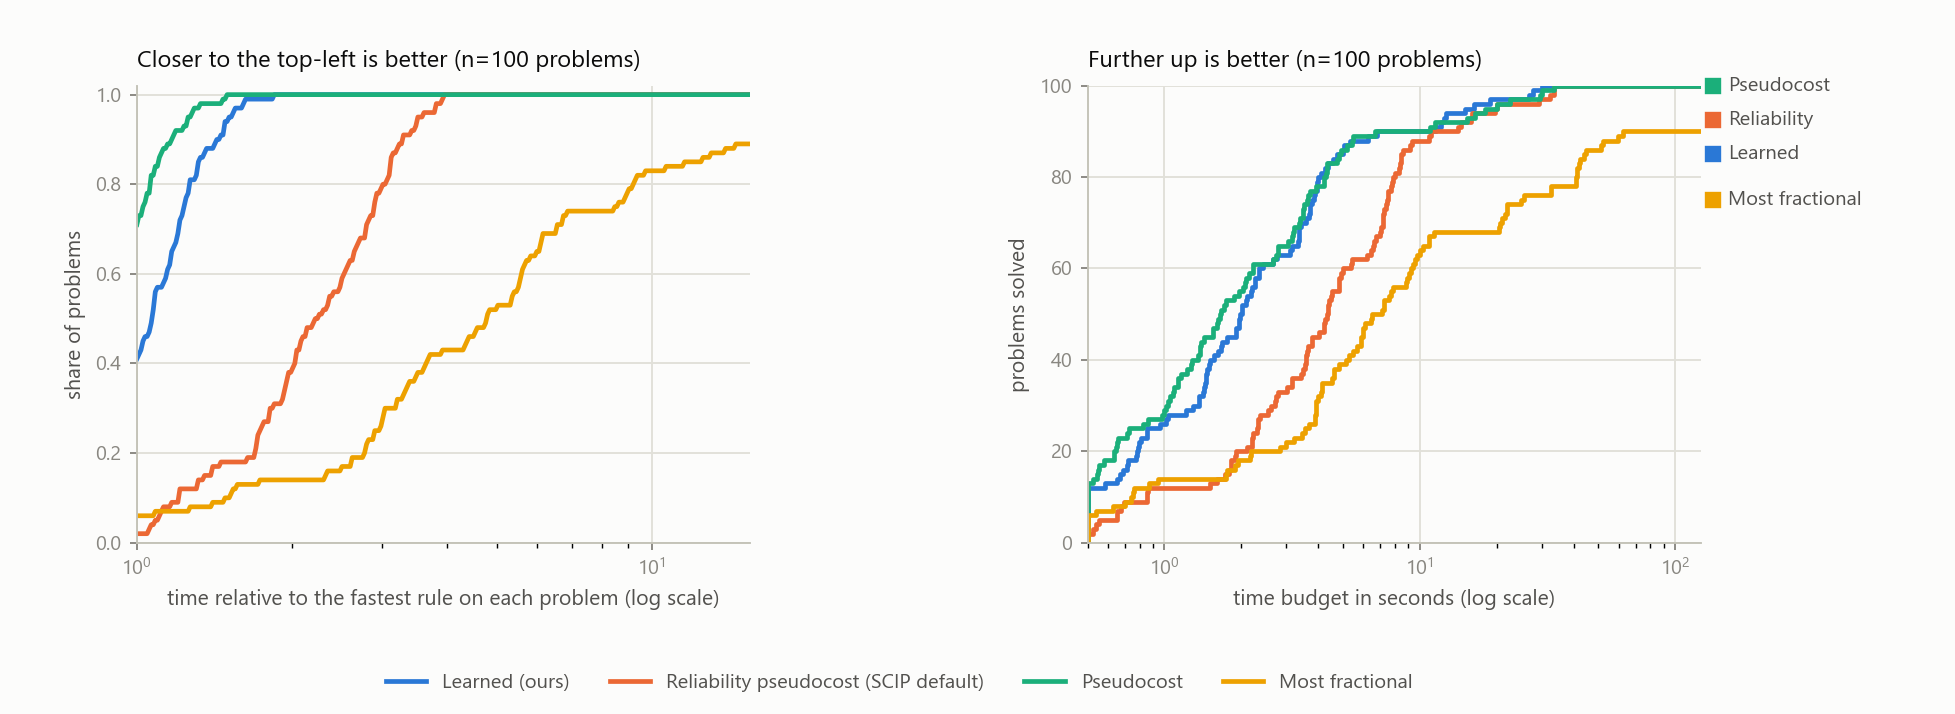
\includegraphics[width=\linewidth]{figures/test_profile.png}
\caption{Test instances. Left: performance profile (share of problems solved within a factor of the best rule's time). Right: problems solved within a time budget. Both axes of time are logarithmic.}
\label{fig:test}
\end{figure}
 
\subsection{Generalization to larger instances}
Trained only on instances with $500$ rows, the model is applied unchanged to instances with $750$ rows (Table~\ref{tab:transfer}, Figure~\ref{fig:transfer}). The picture is the same as on the test set, with a smaller gap to pseudocost: learned versus reliability has time ratio $0.61$ ($[0.54,0.68]$) at $2.1\times$ the nodes, and learned versus pseudocost has ratio $1.03$ ($[0.99,1.08]$), no clear difference, at $0.79\times$ the nodes. The node saving against pseudocost is essentially unchanged ($0.77\times$ on the test set, $0.79\times$ here); the smaller time gap is consistent with a lower relative overhead on larger instances ($8.0\%$ rather than $11.7\%$, Section~\ref{sec:overhead}), but we did not isolate the cause.
 
\begin{table}[t]
\centering
\caption{Larger unseen instances ($30$ instances $\times$ $2$ seeds, $120$\,s).}
\label{tab:transfer}
\begin{tabular}{lcrrr}
\toprule
Rule & Solved & SGM time (s) & SGM nodes & Fastest\\
\midrule
Learned                & 60/60 & 10.05 & 1138 & 36\\
Reliability pseudocost & 60/60 & 15.93 & 634  & 5\\
Pseudocost             & 60/60 & \textbf{9.85} & 1420 & \textbf{41}\\
\bottomrule
\end{tabular}
\end{table}
 
\begin{figure}[t]
\centering
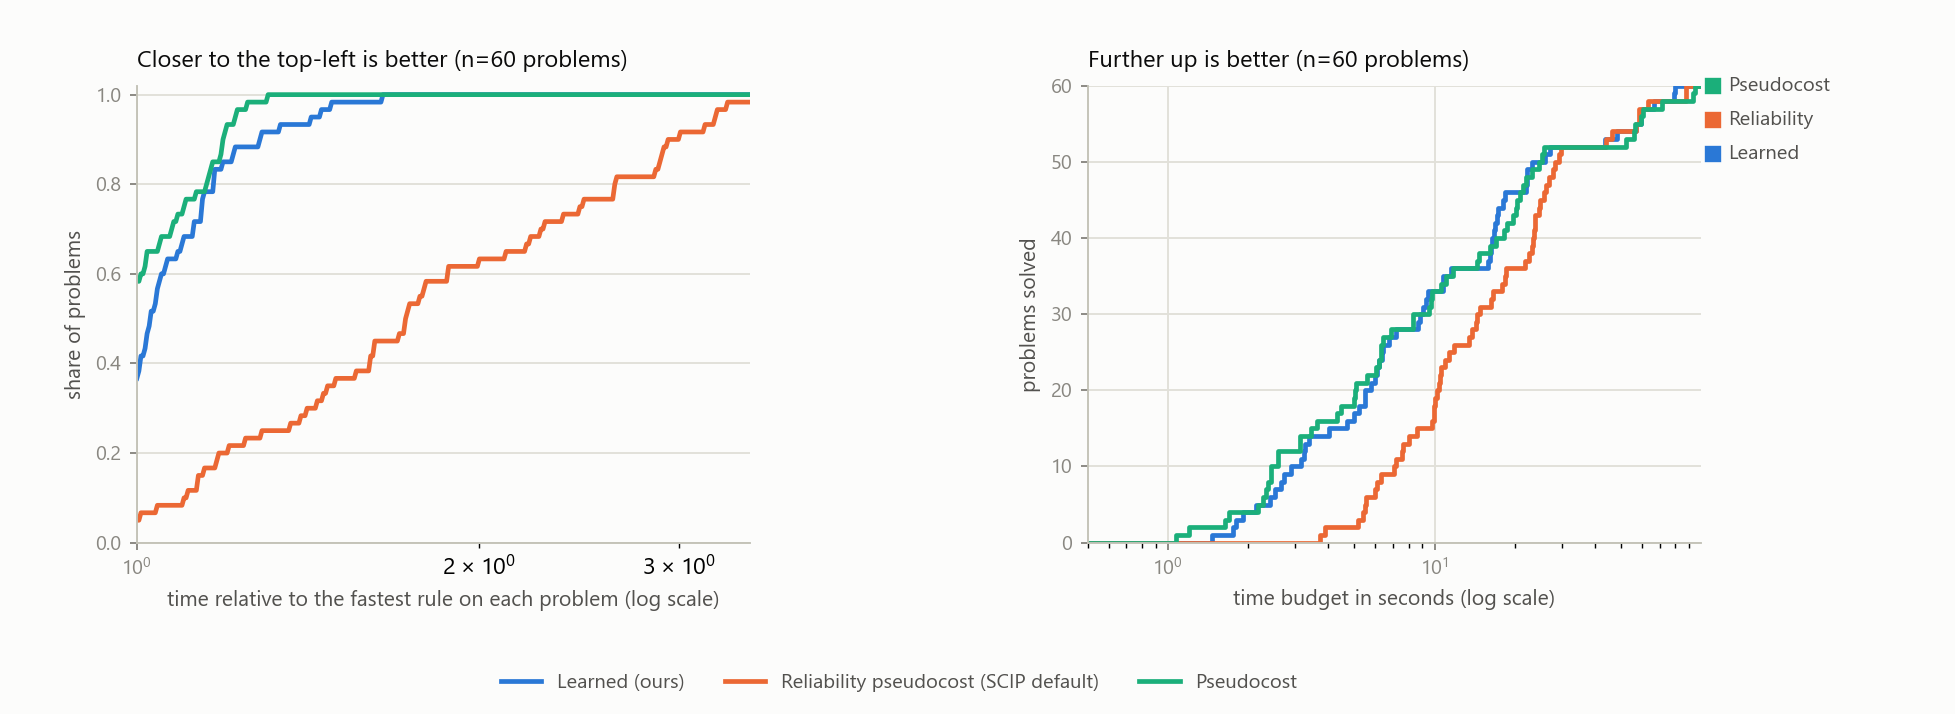
\includegraphics[width=\linewidth]{figures/transfer_profile.png}
\caption{Larger unseen instances ($120$\,s limit); same panels as Figure~\ref{fig:test}.}
\label{fig:transfer}
\end{figure}
 
\subsection{Tight time budget and optimality gap}
With a $120$\,s limit nearly every run is solved, so the optimality gap is uninformative. With a $10$\,s limit on the larger instances (Table~\ref{tab:budget}, Figure~\ref{fig:budget}) the learned rule solves $16$ of $30$ instances, against $9$ for reliability pseudocost branching, and its average gap over all runs is less than half ($2.83\%$ vs.\ $6.15\%$). It matches pseudocost branching (also $16$ solved; $2.98\%$); the $0.15$-point gap difference is within what noise would produce and was not tested. Time ratios here are distorted by the $10$\,s cap (learned versus reliability $0.75$, $[0.66,0.86]$; learned versus pseudocost $1.08$, $[1.02,1.14]$). Only one seed was run.
 
\begin{table}[t]
\centering
\caption{Larger instances with a $10$\,s limit ($30$ instances, seed $0$). Gap: solved runs count as $0$.}
\label{tab:budget}
\begin{tabular}{lccc}
\toprule
Rule & Solved & Avg.\ gap, all runs & Avg.\ gap, unsolved runs\\
\midrule
Learned                & 16/30 & \textbf{2.83\%} & \textbf{6.06\%}\\
Reliability pseudocost & 9/30  & 6.15\% & 8.78\%\\
Pseudocost             & 16/30 & 2.98\% & 6.40\%\\
\bottomrule
\end{tabular}
\end{table}
 
\begin{figure}[t]
\centering
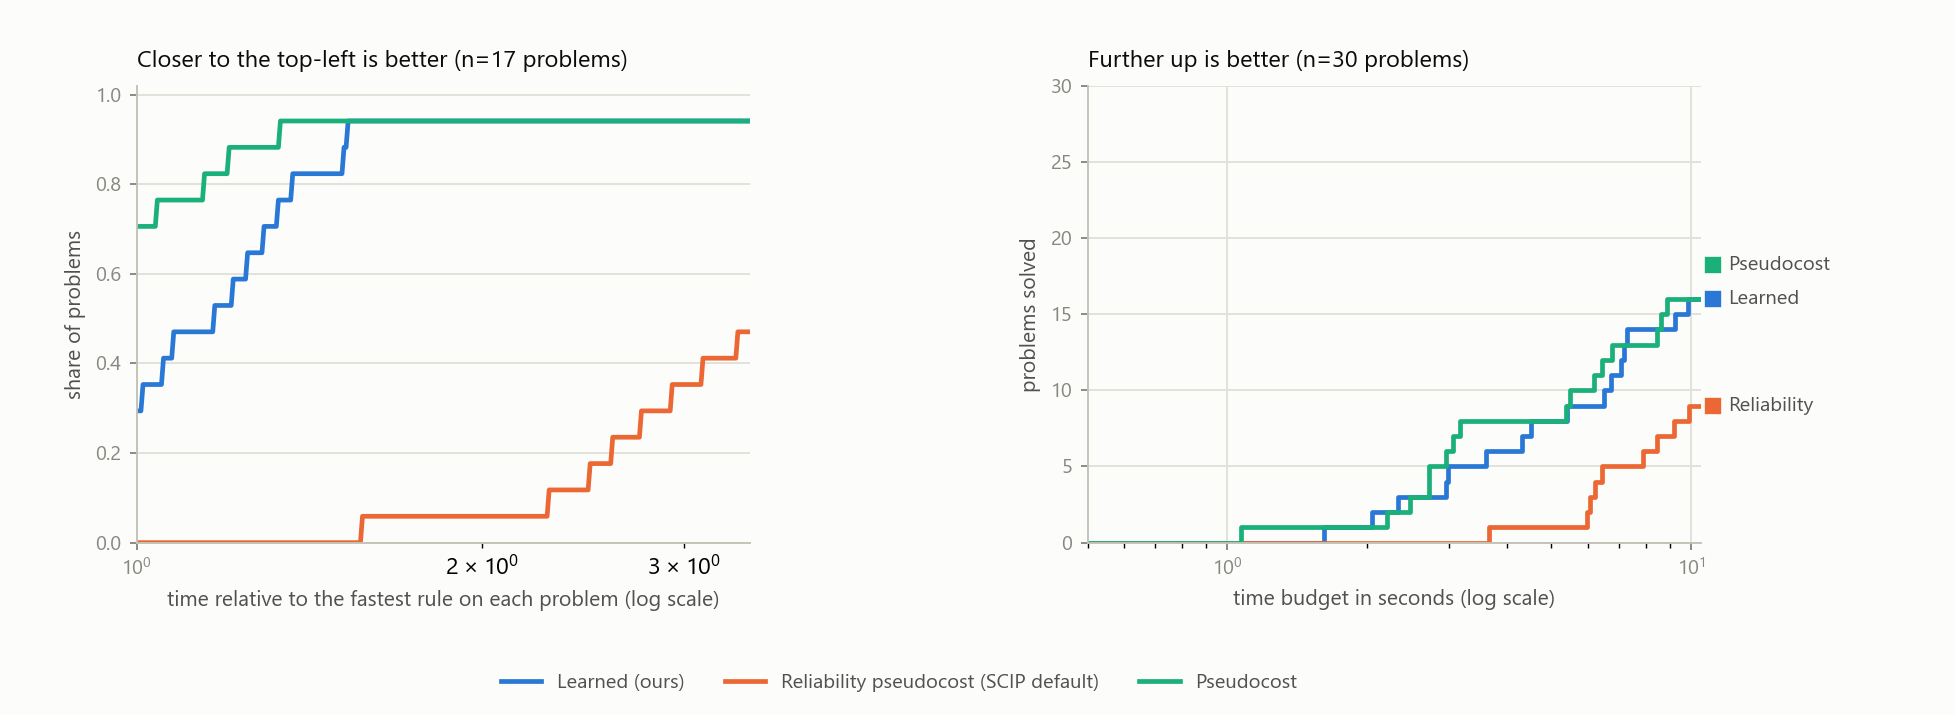
\includegraphics[width=\linewidth]{figures/transfer_10s_profile.png}
\caption{Larger instances, $10$\,s limit, seed $0$; same panels as Figure~\ref{fig:test}. $13$ problems were solved by no rule and are left out of the profile.}
\label{fig:budget}
\end{figure}
 
\subsection{Computational overhead}\label{sec:overhead}
We time feature extraction and model scoring separately from the rest of the callback (which includes SCIP's own call that creates the child nodes, paid by every rule). On the test set the learned rule spends $9.9\%$ of its solve time on feature extraction ($1.29$\,ms per decision) and $1.8\%$ on scoring ($0.23$\,ms), $11.7\%$ in total. On the larger instances with the $10$\,s limit the shares are $6.8\%$ and $1.2\%$ ($1.42$ and $0.26$\,ms), $8.0\%$ in total. Feature extraction is therefore about $85\%$ of the overhead: it consists of many small calls into SCIP from Python, not of model evaluation. This overhead alone does not explain why the learned rule is not faster than pseudocost branching. On the test set the time ratio to pseudocost is $1.09$ for $0.77\times$ the nodes, so a node of the learned rule's tree costs roughly $40\%$ more time ($1.09/0.77$). The measured overhead accounts for a factor of $1/(1-0.117)\approx 1.13$ of that; the remaining factor of about $1.25$ must come from elsewhere. (This is a rough estimate: the time ratio is taken over all $100$ problems, the node ratio over the $90$ solved by every rule.) We did not record LP iterations, so we cannot say whether the learned rule's branching choices lead to more expensive node LPs. Even if the overhead were removed entirely, this back-of-the-envelope estimate gives a time ratio of about $1.09\times0.883\approx 0.96$ on the test set, i.e.\ at most a few percent faster than pseudocost branching.
 
\section{Discussion and limitations}
\paragraph{What the results support.} Under our protocol, a model trained on $300$ small instances to imitate strong branching beats both most-fractional and reliability pseudocost branching in wall-clock time, also on larger instances it never saw, and it builds consistently smaller trees than pseudocost branching. We do not claim it improves on pseudocost branching in time; it does not.
\paragraph{Why not more?} The learned scores largely refine pseudocost information (Section~\ref{sec:offline}), so a large improvement over a pseudocost rule is not expected. Lowering the overhead---caching static features such as objective coefficients and column degrees, computing the fixed-variable fraction incrementally, or a native implementation---can only recover the measured $8$--$12\%$, which by the estimate of Section~\ref{sec:overhead} would give roughly parity to a few percent of speed-up. The unexplained extra cost per node should be diagnosed first (e.g.\ by recording simplex iterations per node). Richer inputs such as graph neural networks \citep{gasse2019exact} are a separate direction.
\paragraph{Limitations.} (i)~A single problem class, set covering; no claim is made for other classes. (ii)~Cuts, presolve and restarts are disabled, so the results say nothing about SCIP with its default settings, where reliability branching is used together with these components. (iii)~Only two seeds; two parallel workers, hence noisy timings. (iv)~Validation instances were used for early stopping. (v)~Training labels come from strong branching on a random subset of at most $60$ candidates per node, and the model scores all candidates at test time. (vi)~The tight-budget experiment uses one seed, and the gap comparison with pseudocost was not tested.
 
\section{Conclusion}
A gradient-boosted ranker trained to imitate strong branching, using cheap features, gives a branching rule that is substantially faster than reliability pseudocost and most-fractional branching in our setup and generalizes from $500$ to $750$ rows, but does not beat plain pseudocost branching in solve time: its trees are about $20\%$ smaller, yet each node costs more, partly because of feature extraction. Measuring time and overhead explicitly, rather than node counts alone, is what makes the comparison honest.
 
\bibliographystyle{plainnat}
\bibliography{references}
 
\end{document}
 